\documentclass[10pt]{article}
\usepackage{../pplmanual}
%%% Commonly Needed packages
\usepackage{graphicx,color,calc}
\usepackage{fancyvrb}
\usepackage{makeidx}
\usepackage{alltt}
\usepackage[linkbordercolor=(0 0 1),citebordercolor=(0 1 0)]{hyperref}
%%\usepackage{xspace} <- creates problems with other hyperlink packages like "html"

%%% Commands for uniform looks of C++, Charm++, and Projections
\newcommand{\CC}{C\hbox{++}}
\newcommand{\emCC}{C\hbox{\em++}}
\newcommand{\charmpp}{\textsc{Charm++}}
\newcommand{\charmc}{\texttt{charmc}}
\newcommand{\projections}{\textsc{Projections}}
\newcommand{\converse}{\textsc{Converse}}
\newcommand{\ampi}{\textsc{AMPI}}
\newcommand{\tempo}{\textsc{TeMPO}}
\newcommand{\irecv}{\textsl{iRecv}}
\newcommand{\sdag}{\textsl{Structured Dagger}}
\newcommand{\jade}{Jade}

%%% Commands to produce margin symbols
\newcommand{\new}{\marginpar{\fbox{\bf$\mathcal{NEW}$}}}
\newcommand{\important}{\marginpar{\fbox{\bf\Huge !}}}
\newcommand{\experimental}{\marginpar{\fbox{\bf\Huge $\beta$}}}

%%% Commands for manual elements
\newcommand{\zap}[1]{ }
\newcommand{\function}[1]{{\noindent{\textsf{#1}}\\}}
\newcommand{\cmd}[1]{{\noindent{\textsf{#1}}\\}}
\newcommand{\args}[1]{\hspace*{2em}{\texttt{#1}}\\}
\newcommand{\prototype}[1]{\vspace{0.2in}\index{#1}}
\newcommand{\param}[1]{{\texttt{#1}}}
\newcommand{\kw}[1]{{\textsf{#1}\index{#1}}}
\newcommand{\uw}[1]{{\textsl{#1}}}
\newcommand{\desc}[1]{\indent{#1}}
\newcommand{\note}[1]{(\textbf{Note:} #1)}
\newcommand{\term}[1]{{\bf #1}\index{#1}}

\makeindex


\makeindex

\title{\charmpp\\ NetFEM\\ Manual}
\version{1.0}
\credits{
The initial version of \charmpp{} NetFEM Framework was developed
by Orion Lawlor in 2001.
}

\begin{document}

\maketitle

\section{Introduction}

NetFEM was built to provide an easy way to visualize
the current state of a finite-element simulation, or any 
parallel program that computes on an unstructured mesh.
NetFEM is designed to require very little effort to add
to a program, and connects to the running program over
the network via the network protocol CCS (Converse Client/Server).


\section{Compiling and Installing}

NetFEM is part of \charmpp{}, so it can be downloaded
as part of charm.  To build NetFEM, just build FEM normally,
or else do a make in charm/netlrts-linux/tmp/libs/ck-libs/netfem/.

To link with NetFEM, add \kw{-module netfem} to your
program's link line.  Note that you do {\em not} need to use
the FEM framework to use NetFEM.

The netfem header file for C is called ``netfem.h'',
the header for fortran is called `netfemf.h'.
A simple example NetFEM program is in 
  charm/pgms/charm++/fem/simple2D/.
A more complicated example is in
  charm/pgms/charm++/fem/crack2D/.


\section{Running NetFEM Online}

Once you have a NetFEM program, you can run it and view 
the results online by starting the program with CCS enabled:

\begin{verbatim}
   foo.bar.edu>  ./charmrun ./myprogram +p2 ++server ++server-port 1234
\end{verbatim}

``++server-port'' controls the TCP port number to use for CCS---here,
we use 1234.  Currently, NetFEM only works with one chunk per
processor---that is, the -vp option cannot be used.

To view the results online, you then start the NetFEM client, 
which can be downloaded for Linux or Windows from 

\begin{verbatim}
http://charm.cs.uiuc.edu/research/fem/netfem/
\end{verbatim}

Enter the name of the machine running charmrun and
the TCP port number into the NetFEM client---for example, 
you might run:

\begin{verbatim}
  netfem foo.bar.edu:1234
\end{verbatim}

The NetFEM client will then connect to the program,
download the most recent mesh registered with 
\kw{NetFEM\_POINTAT}, and display it.
At any time, you can press the ``update'' button 
to reload the latest mesh.


\section{Running NetFEM Offline}

Rather than using CCS as above, you can register your meshes
using \kw{NetFEM\_WRITE}, which makes the server write out 
binary output dump files.  For example, to view timestep 10,
which is written to the ``NetFEM/10/`` directory, you'd 
run the client program as:

\begin{verbatim}
  netfem NetFEM/10
\end{verbatim}

In offline mode, the ``update'' button fetches the next
extant timestep directory.

\section{NetFEM with other Visualization Tools}

You can use a provided converter program to convert the offline NetFEM files into an XML format compatible with the powerful offline visualization tool ParaView(\url{http://paraview.org}). The converter is located in .../charm/src/libs/ck-libs/netfem/ParaviewConverter/. Build the converter by simply issuing a ``make'' command in that directory(assuming NetFEM already has been built).



Run the converter from the parent directory of the "NetFEM" directory to be converted. The converter will generate a directory called ``ParaViewData'', which contains subdirectories for each timestep, along with a ``timestep''directory for index files for each timestep. All files in the ParaViewData directory can be opened by ParaView. To open all chunks for a given timestep, open the desired timestep file in ``ParaViewData/timesteps''. Also, individual partition files can also be opened from ``ParaViewData / $<$timestep$>$ / $<$partition\_num$>$''.



\section{Interface Basics}

You publish your data via NetFEM by making a series of
calls to describe the current state of your data.  
There are only 6 possible calls you can make.

\kw{NetFEM\_Begin} is the first routine you call.
\kw{NetFEM\_End} is the last routine to call.  These
two calls bracket all the other NetFEM calls.

\kw{NetFEM\_Nodes} describes the properties of the
nodes, or vertices of the domain.  \kw{NetFEM\_Elements}
describes the properties of your elements (triangles,
tetrahedra, etc.).  After making one of these calls,
you list the different data arrays associated with your 
nodes or elements by making calls to \kw{NetFEM\_Scalar} 
or \kw{NetFEM\_Vector}.

For example, a typical finite element simulation might
have a scalar mass and vector position, velocity, and net force
associated with each node; and have a scalar stress value
associated with each element.  The sequence of NetFEM calls
this application would make would be:

\begin{verbatim}
  NetFEM_Begin
    NetFEM_Nodes -- lists position of each node
      NetFEM_Vector -- lists velocity of each node
      NetFEM_Vector -- lists net force on each node
      NetFEM_Scalar -- lists mass of each node
    
    NetFEM_Elements -- lists the nodes of each element
      NetFEM_Scalar -- lists the stress of each element
  
  NetFEM_End
\end{verbatim}

\begin{figure}[h]
\begin{center}
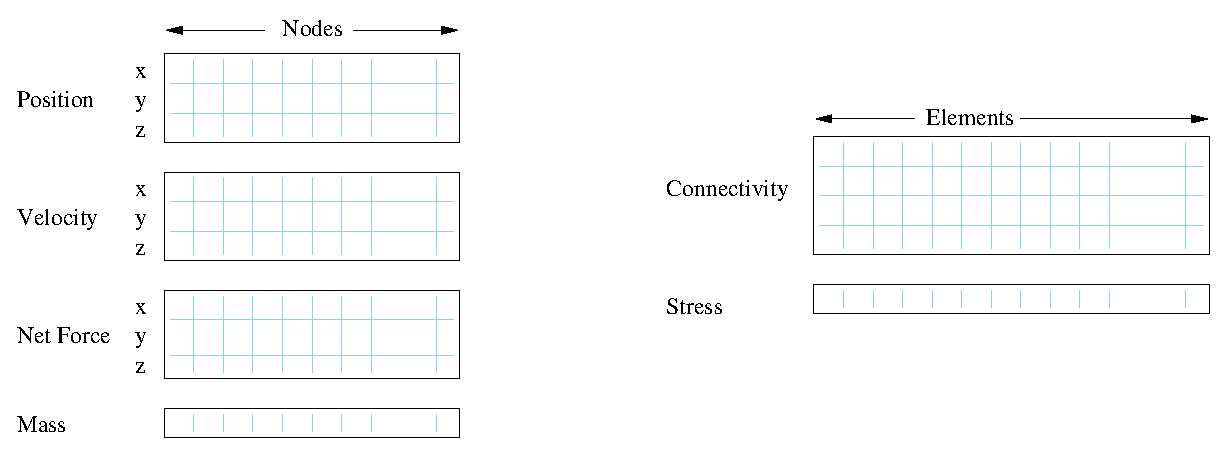
\includegraphics[width=5in]{fig/example}
\end{center}
\caption{These arrays, typical of a finite element analysis
program, might be passed into NetFEM.}
\label{fig:example}
\end{figure}


\section{Simple Interface}
The details of how to make each call are:

\prototype{NetFEM\_Begin}
\function{NetFEM NetFEM\_Begin(int source, int step, int dim, int flavor);}
\function{integer function NetFEM\_Begin(source,step,dim,flavor)}
  \args{integer, intent(in)  :: source,step,dim,flavor}

Begins describing a single piece of a mesh.  Returns a handle
that is used for each subsequent call until \kw{NetFEM\_End}.  
This call, like all NetFEM calls, is collective---every processor 
should make the same calls in the same order.

\uw{source} identifies the piece of the mesh---use FEM\_My\_partition
or CkMyPe.

\uw{step} identifies which version of the mesh this is---for example,
you might use the timestep number.  This is only used to identify the
mesh in the client.

\uw{dim} is the number of spatial dimensions.  For example, in a 2D
computation, you'd pass dim==2; in a 3D computation, dim==3.
The client currently only supports 2D or 3D computations.

\uw{flavor} specifies what to do with the data.  This can
take the value \kw{NetFEM\_POINTAT}, which is used in online visualization,
and specifies that NetFEM should only keep a pointer to your data 
rather than copy it out of your arrays.  Or it can take the value
\kw{NetFEM\_WRITE}, which writes out the data to files named
``NetFEM/\uw{step}/\uw{source}.dat'' for offline visualization. 


\prototype{NetFEM\_End}
\function{void NetFEM\_End(NetFEM n);}
\function{subroutine NetFEM\_End(n)}
  \args{integer, intent(in)  :: n}

Finishes describing a single piece of a mesh, which 
then makes the mesh available for display.


\prototype{NetFEM\_Nodes}
\function{void NetFEM\_Nodes(NetFEM n,int nNodes,const double *loc,const char *name);}
\function{subroutine NetFEM\_Nodes(n,nNodes,loc,name)}
  \args{integer, intent(in)  :: n, nNodes}
  \args{double precision, intent(in)  :: loc(dim,nNodes) }
  \args{character*(*), intent(in)  :: name}

Describes the nodes in this piece of the mesh.

\uw{n} is the NetFEM handle obtained from \kw{NetFEM\_Begin}.

\uw{nNodes} is the number of nodes listed here.

\uw{loc} is the location of each node.  This must be double-precision
array, laid out with the same number of dimensions as passed to 
\kw{NetFEM\_Begin}.  For example, in C the location of a 2D
node $n$ is stored in loc[2*n+0] (x coordinate) and loc[2*n+1]
(y coordinate).  In Fortran, location of a node $n$ is stored 
in loc(:,n).

\uw{name} is a human-readable name for the node locations
to display in the client.  We recommend also including the location
units here, for example "Position (m)".


\prototype{NetFEM\_Elements}
\function{void NetFEM\_Elements(NetFEM n,int nElements,int nodePerEl,const int *conn,const char *name);}
\function{subroutine NetFEM\_Elements(n,nElements,nodePerEl,conn,name)}
  \args{integer, intent(in)  :: n, nElements, nodePerEl}
  \args{integer, intent(in)  :: conn(nodePerEl,nElements) }
  \args{character*(*), intent(in)  :: name}

Describes the elements in this piece of the mesh.
Unlike \kw{NetFEM\_Nodes}, this call can be repeated
if there are different types of elements (For example, 
some meshes contain a mix of triangles and quadrilaterals).

\uw{n} is the NetFEM handle obtained from \kw{NetFEM\_Begin}.

\uw{nElements} is the number of elements listed here.

\uw{nodePerEl} is the number of nodes for each element.
For example, a triangle has 3 nodes per element; while 
tetrahedra have 4.

\uw{conn} gives the index of each element's nodes.  Note
that when called from C, the first node is listed in 
\uw{conn} as 0 (0-based node indexing), and element $e$'s
first node is stored in conn[e*nodePerEl+0].
When called from Fortran, the first node is listed as 1 
(1-based node indexing), and element $e$'s first node is
stored in conn(1,e) or conn((e-1)*nodePerEl+1).

\uw{name} is a human-readable name for the elements
to display in the client.  For example, this might be
"Linear-Strain Triangles".



\prototype{NetFEM\_Vector}
\function{void NetFEM\_Vector(NetFEM n,const double *data,const char *name);}
\function{subroutine NetFEM\_Vector(n,data,name)}
  \args{integer, intent(in)  :: n}
  \args{double precision, intent(in)  :: data(dim,lastEntity) }
  \args{character*(*), intent(in)  :: name}

Describes a spatial vector associated with each node or element
in the mesh.  Attaches the vector to the most recently listed 
node or element.  You can repeat this call several times to 
describe different vectors.

\uw{n} is the NetFEM handle obtained from \kw{NetFEM\_Begin}.

\uw{data} is the double-precision array of vector values.
The dimensions of the array have to match up with the node
or element the data is associated with--in C, a 2D element $e$'s
vector starts at data[2*e]; in Fortran, element $e$'s 
vector is data(:,e).

\uw{name} is a human-readable name for this vector data.
For example, this might be "Velocity (m/s)".


\prototype{NetFEM\_Scalar}
\function{void NetFEM\_Scalar(NetFEM n,const double *data,int dataPer,const char *name);}
\function{subroutine NetFEM\_Scalar(n,data,dataPer,name)}
  \args{integer, intent(in)  :: n, dataPer}
  \args{double precision, intent(in)  :: data(dataPer,lastEntity) }
  \args{character*(*), intent(in)  :: name}

Describes some scalar data associated with each node or element
in the mesh.  Like \kw{NetFEM\_Vector}, this data is attached 
to the most recently listed node or element and this call 
can be repeated.  For a node or element, you can make the 
calls to \kw{NetFEM\_Vector} and \kw{NetFEM\_Scalar} in any order.

\uw{n} is the NetFEM handle obtained from \kw{NetFEM\_Begin}.

\uw{data} is the double-precision array of values.
In C, an element $e$'s scalar values start at data[dataPer*e];
in Fortran, element $e$'s values are in data(:,e).

\uw{dataPer} is the number of values associated with each 
node or element.  For true scalar data, this is 1; but 
can be any value.  Even if dataPer happens to equal the number
of dimensions, the client knows that this data does not 
represent a spatial vector.

\uw{name} is a human-readable name for this scalar data.
For example, this might be "Mass (Kg)" or "Stresses (pure)".



\section{Advanced ``Field'' Interface}
This more advanced interface can be used if you 
store your node or element data in arrays of C structs or 
Fortran TYPEs.  To use this interface, you'll have to
provide the name of your struct and field.  Each
``field'' routine is just an extended version of 
a regular NetFEM call described above, and can be 
used in place of the regular NetFEM call.
In each case, you pass a description of your field
in addition to the usual NetFEM parameters.

In C, use the macro ``NetFEM\_Field(theStruct,theField)''
to describe the FIELD.  For example, to describe
the field ``loc'' of your structure named ``node\_t'',

\begin{verbatim}
   node\_t *myNodes=...;
   ..., NetFEM\_Field(node\_t,loc), ...
\end{verbatim}


In Fortran, you must pass as FIELD the byte offset from the start 
of the structure to the start of the field,
then the size of the structure.  The FEM "foffsetof" routine,
which returns the number of bytes between its arguments,
can be used for this.  For example, to describe the field
``loc'' of your named type ``NODE'',

\begin{verbatim}
   TYPE(NODE), ALLOCATABLE :: n(:)
   ..., foffsetof(n(1),n(1)%loc),foffsetof(n(1),n(2)), ...
\end{verbatim}


\prototype{NetFEM\_Nodes\_field}
\function{void NetFEM\_Nodes\_field(NetFEM n,int nNodes,FIELD,const void *loc,const char *name);}
\function{subroutine NetFEM\_Nodes\_field(n,nNodes,FIELD,loc,name)}

A FIELD version of \kw{NetFEM\_Nodes}.

\prototype{NetFEM\_Elements\_field}
\function{void NetFEM\_Elements\_field(NetFEM n,int nElements,int nodePerEl,FIELD,int idxBase,const int *conn,const char *name);}
\function{subroutine NetFEM\_Elements\_field(n,nElements,nodePerEl,FIELD,idxBase,conn,name)}

A FIELD version of \kw{NetFEM\_Elements}.
This version also allows you to control the starting node
index of the connectivity array---in C, this is normally 0;
in Fortran, this is normally 1.

\prototype{NetFEM\_Vector\_field}
\function{void NetFEM\_Vector\_field(NetFEM n,const double *data,FIELD,const char *name);}
\function{subroutine NetFEM\_Vector\_field(n,data,FIELD,name)}

A FIELD version of \kw{NetFEM\_Vector}.


\prototype{NetFEM\_Scalar\_field}
\function{void NetFEM\_Scalar\_field(NetFEM n,const double *data,int dataPer,FIELD,const char *name);}
\function{subroutine NetFEM\_Scalar(n,data,dataPer,FIELD,name)}

A FIELD version of \kw{NetFEM\_Scalar}.


\end{document}
